\documentclass[aspectratio=169]{beamer}
\usepackage{amsmath}
\usepackage{amssymb}
\usepackage{amsfonts}
\usepackage{graphicx}
\usepackage{luatexja} 
\usepackage{comment}
\usepackage{bm}
\usepackage{setspace}
\usepackage{caption}

\usetheme{LightTheme}
\setbeamertemplate{footline}[frame number]
\setbeamertemplate{navigation symbols}{}
\setlength{\baselineskip}{10pt}
\begin{document}

% タイトルフレーム
\title{\Large 木幅アルゴリズムの学習システムの構築}
\subtitle{進捗状況} 
\author{\small B4 小林紹子} % 必要に応じて変更・削除
\date{\small\today} % 必要に応じて変更・削除

\begin{frame}
    \titlepage
\end{frame}

\begin{frame}{目次}
    \tableofcontents
\end{frame}

\section{学習システム構築の目的}

\begin{frame}{研究背景}
    \begin{itemize}
        \setlength{\parskip}{1.5em}
        \item 木幅はグラフ構造理論などアルゴリズム設計で重要な概念.
        \item しかし,
        \begin{itemize}
            \setlength{\parskip}{1em}
            \item 理解が難しい(抽象的な概念,木分解の構築の難しさ)
            \item 日本語で学べる教材や可視化・インタラクティブな教材が少ない.
        \end{itemize}
        \item \Rightarrow 「木幅アルゴリズムを直感的に学べる教材」が求められている.
    \end{itemize}
\end{frame}

\begin{frame}{研究目的}
    \begin{itemize}
        \setlength{\parskip}{1.5em}
        \item 木幅や木分解の理解を支援する学習サイトを開発する.
        \item 対象:アルゴリズムをある程度学習している人(例:情報系学生).
        \item 目的:
        \begin{itemize}
            \setlength{\parskip}{1.5em}
            \item 定義の理解促進.
            \item アルゴリズムの可視化による直感的理解.
        \end{itemize}
    \end{itemize}
\end{frame}

\section{要件定義}

\begin{frame}[allowframebreaks]{要件定義}
    \begin{enumerate}
        \setlength{\parskip}{1em}
        \item 問題管理機能(サーバー側)
        \begin{itemize}
            \item 問題文,画像,正答を含む問題データを保持.
            \item API経由でデータのやり取りを行う.
        \end{itemize}
        \item 問題表示機能(クライアント側)
        \begin{itemize}
            \item サーバーから問題リストを取得して表示.
            \item 問題文と対応する画像の表示.
            \item ユーザーが解答を選択・入力可能.
        \end{itemize}
        \newpage
        \item 解答送信・結果表示機能
        \begin{itemize}
            \item 解答送信時にサーバーにリクエストを送信.
            \item サーバー側で判定し,結果を返す.
            \item ページ遷移せずに喧嘩を即時表示.
        \end{itemize}
        \item インタラクティブに図をマウス等で操作.
        \begin{itemize}
            \item 操作し変更された図の頂点をデータとして保持.
            \item 解答として送信可能.
        \end{itemize}
        \item 相手の解答パターンに合わせた正解を自動生成.
        \begin{itemize}
            \item それ以前に選択された答えによって異なる解答が得られる.
            \item サーバー側でインタラクティブに生成.
        \end{itemize}
    \end{enumerate}
\end{frame}

\begin{frame}{将来的な拡張要件}
    \begin{itemize}
        \setlength{\parskip}{1.5em}
        \item 管理者画面での問題追加・削除.
        \item ユーザー登録.
        \item 回答履歴・正答率の記録.
    \end{itemize}
\end{frame}

\section{Webアプリケーション}

\begin{frame}{このまま説明する前に}
    \begin{itemize}
        \setlength{\parskip}{1.5em}
        \item これから使用技術について説明したい.
        \item 事前に説明してみたら,井口先生にウェブプログラミングを履修していない学生が多いと言われた.
        \item 今後のためにもまずは基本的なWebアプリケーションについての仕組みを説明します...
    \end{itemize}
\end{frame}
\begin{frame}{WebアプリケーションとWebサイトの違い}
    \begin{itemize}
        \setlength{\parskip}{1.5em}
        \item \textbf{Webサイト}:常に同じHTMLをクライアントに返す.
        \item \textbf{Webアプリケーション}:\\表示内容をクライアントごとに動的に変化するHTMLを返す.
        \begin{enumerate}
            \setlength{\parskip}{1em}
            \item WebブラウザからURLを入力してEnter.\\リクエスト情報がWebアプリに送信(リクエスト).
            \item リクエストがWebアプリに届くと,リソース(HTML, CSS)をデータベースと連携して取得.
            \item ブラウザに返す(レスポンス).
        \end{enumerate}
    \end{itemize}
\end{frame}

\begin{frame}{サーバーとクライアント}
    
\end{frame}
\end{document}
\begin{frame}{学習システム構築の目的}
    \begin{itemize}
        \setlength{\itemsep}{2em}
        \item 
    \end{itemize}
\end{frame}

\begin{frame}{memo関数とuseCallbackの関係}
    \begin{itemize}
        \setlength{\itemsep}{2em}
        \item memo関数
        \begin{itemize}
            \item propsが同じであれば再描画をスキップする.
        \end{itemize}
        \item useCallback
        \begin{itemize}
            \item 関数の参照をメモ化.
            \item 依存配列が変わらない限り,同じ関数オブジェクトを再利用.
            \item 再レンダーされても「新しい関数が作られる」ことはない.
        \end{itemize}
    \end{itemize} 
    \rightarrowfill useCallbackとmemo関数を同時に使うことで再描画を防げる.

\end{frame}
\begin{frame}
    \begin{figure}
        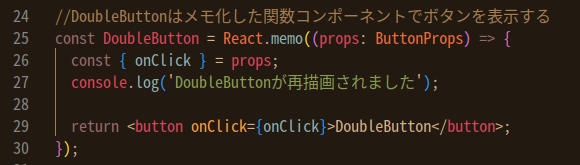
\includegraphics[scale = 0.5]{useCallback1.png}
    \end{figure}
    \begin{figure}
        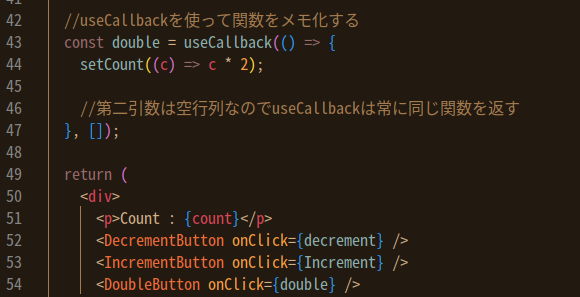
\includegraphics[scale = 0.5]{useCallback2.png}
    \end{figure}
\end{frame}

\section{Next.jsとReact}

\begin{frame}[allowframebreaks]{Next.jsとReact}
    \begin{itemize}
        \setlength{\itemsep}{2em}
        \item Next.js : Reactをベースに開発されたフレームワーク.
        \item React : Javascriptにおけるライブラリの一つ.
    \end{itemize}
    \vspace{2em}
    ライブラリ:\\開発時に使われるコードの集まり.作業を簡略化するための関数や定義・クラスの集まり.\\
    フレームワーク:\\テンプレートのようなもの.ログイン機能や決算機能など必要な機能がデフォルトで揃っている.\\
    \Rightarrow Next.jsはReactライブラリのフレームワーク
    \begin{figure}
        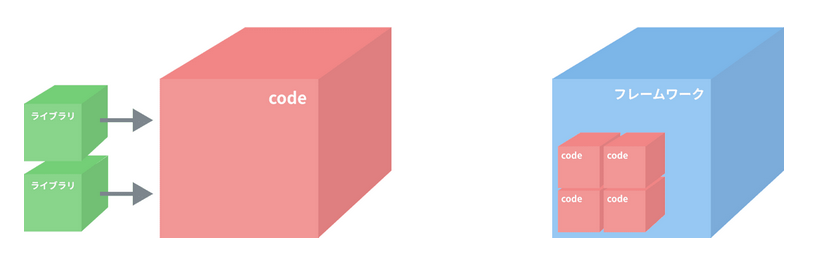
\includegraphics[scale=0.5]{Next.js_and_React.png}
        \caption{ReactとNext.js}
    \end{figure}
\end{frame}

\begin{frame}[allowframebreaks]{Next.jsの特徴}
    \begin{itemize}
        \item RCS(React Server Components)
        \begin{itemize}
             \setlength{\itemsep}{2em}
            \item Reactは従来SSR(Server Side Rendering)を行ってきた.
            \item SSR : 全てのコンポーネントをサーバーでHTMLに変換する.
            \item RCSでは、それをサーバーで実行する部分とクライアントで実行する部分を分けることができる.
            \item これにより,無駄なリロードが減る.
        \end{itemize}
        \newpage
        \item App Router
        \begin{itemize}
            \item ディレクトリ構造がそのままURLの構造になる.
            \item ルーティングは/app配下のディレクトリベースで行う.
            \item page.tsxでルートの画面,router.tsxでAPIエンドポイントを書くなどファイル規約がある.
            \begin{figure}
                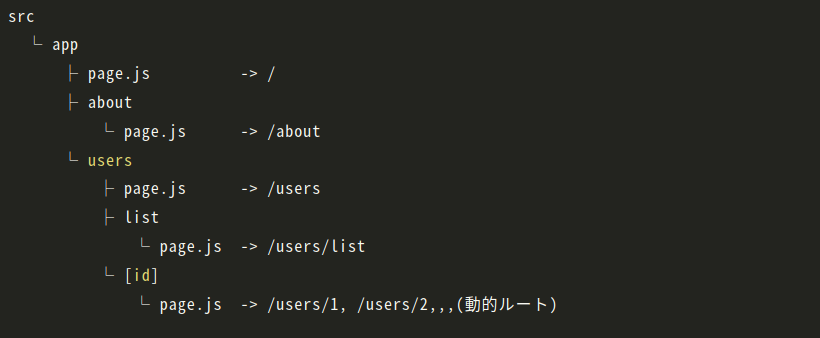
\includegraphics[scale=0.35]{AppRouter.png}
            \end{figure}
        \end{itemize}
    \end{itemize}
\end{frame}

\section{作業経過}
\begin{frame}{環境構築}
    \begin{itemize}
        \setlength{\itemsep}{1em}
        \item npmをインストール(sudo apt npm)version : v22.15.0
        \item Next.jsをインストール(npx create-next-app@latest --ts next-sample)version:v22.15.0
        \item ここでTurbopackが開発サーバークラッシュしてるとエラーがでた.
        \item \rightarrow nodemoduleとpackage.jsonを削除
        \item npm i で再インストールするとうまくいった.
        \item npm run devで初期画面がでてきた.(http://localhost:3000)
    \end{itemize}    
\end{frame}

\begin{frame}{画面描画}
    \begin{itemize}
        \setlength{\itemsep}{2em}
        \item React Flow : インタラクティブなダイアグラムを簡単に実装できる.
        \item npm install reactflow
        \item 作れはしたが、もともとチャートフロウなどを書く用に作られたものだったので上手な図形は作れず.
    \end{itemize}
\end{frame}

\begin{frame}[allowframebreaks]{コード}
    \begin{figure}
        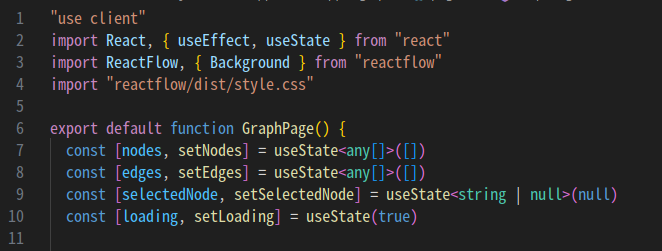
\includegraphics[scale=0.6]{graph1.png}
        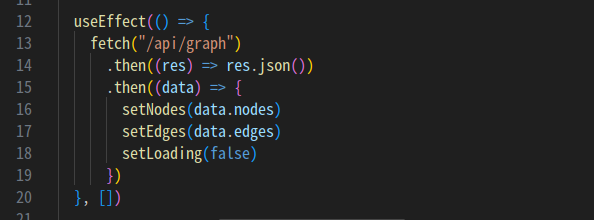
\includegraphics[scale=0.6]{graph2.png}
    \end{figure}
\end{frame}

\begin{frame}{○×問題}
    \begin{itemize}
        \setlength{\itemsep}{2em}
        \item まずはバックエンド・フロントエンドに問題・回答を書いた.
        \item JSONで答えをサーバからもらって判断する.
        \item 将来的にはデータベースから問題を取得するようにする.
    \end{itemize}
\end{frame}

\begin{frame}[allowframebreaks]{フロントエンド(page.tsx)}
    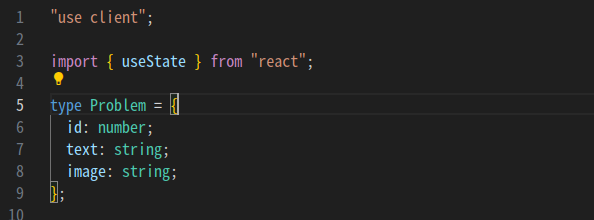
\includegraphics[scale=0.6]{q1.png}
    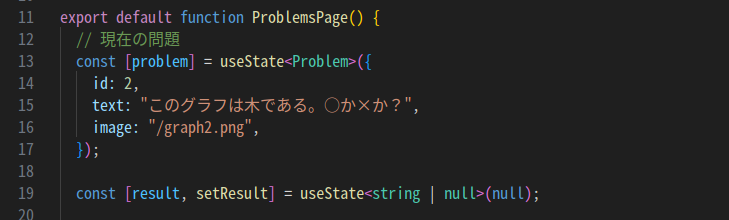
\includegraphics[scale=0.6]{q2.png}
    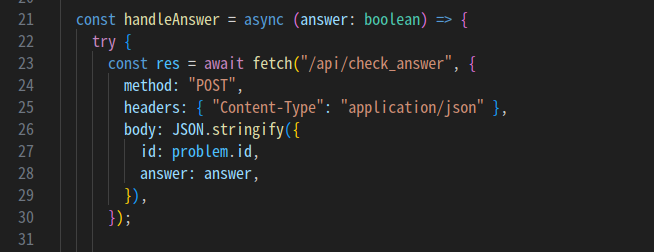
\includegraphics[scale=0.6]{q3.png}
    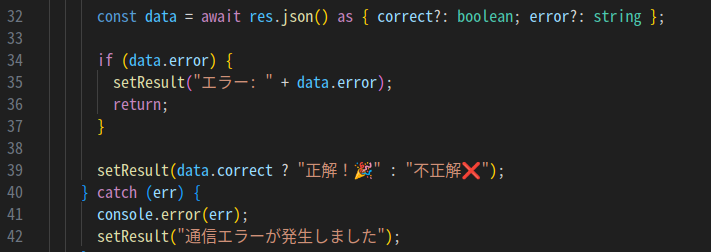
\includegraphics[scale=0.6]{q4.png}
\end{frame}

\begin{frame}[allowframebreaks]{バックエンド(route.tsx)}
    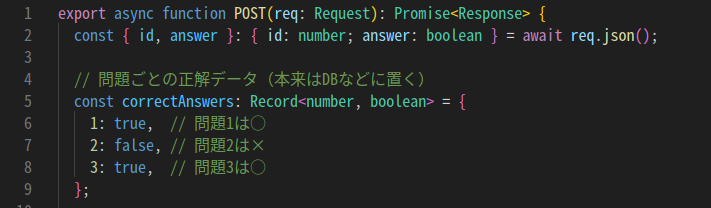
\includegraphics[scale=0.6]{check1.png}
    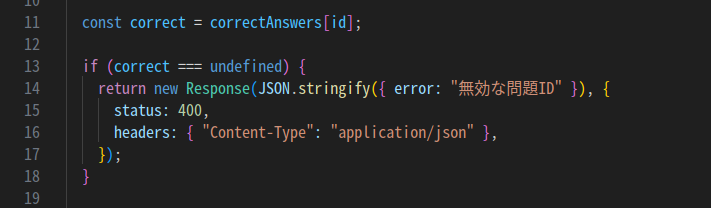
\includegraphics[scale=0.6]{check2.png}
    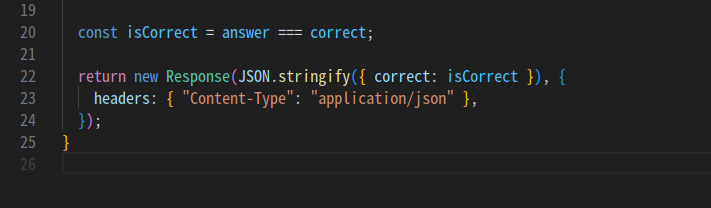
\includegraphics[scale=0.6]{check3.png}
\end{frame}
\end{document}


